\documentclass[../main.tex]{subfiles}
\graphicspath{{\subfix{../figures/}}}
%
\begin{document}
\section{装饰模式(Decoration)}
\noindent 装饰模式又称包装(Wrapper)模式。装饰模式以对客户端透明的方式扩展对象的功能。是继承关系的一种替代方案。
%
\subsection{装饰模式的结构}
装饰模式使用装饰类的一个子类的实例,把客户端的调用委派到其它装饰类或具体构件类。装饰模式的关键在于这种扩展是完全透明的。
%
\begin{figure}[H]
  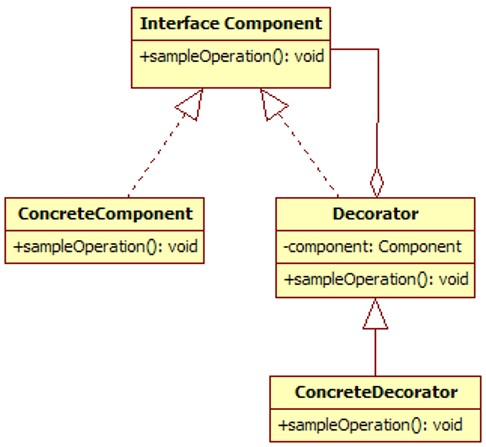
\includegraphics[width=0.55\textwidth]{22_1.jpg}
\end{figure}
%
\textbf{模式中的角色}:
\begin{itemize}
  \item 抽象构件(Component)角色:给出一个接口,以规范准备接收附加责任(扩展功能)的对象。
  \item 具体构件(Concrete Component)角色:定义一个准备接收附加责任的类。
  \item 装饰(Decorator)角色:持有一个构件的实例,并定义与抽象构件接口一致的接口。
  \item 具体装饰(Concrete Decorator)角色:负责给构件对象``贴上''附加的责任。
\end{itemize}
%
下面给出装饰模式的示意性源代码。首先是抽象构件角色的源代码:
%
\lstinputlisting[language=java]{./code/22/1/Component.java}
%
下面是装饰角色的源代码:
%
\lstinputlisting[language=java]{./code/22/1/Decorator.java}
%
应当指出的有以下几点:
\begin{itemize}
  \item 在上面的装饰类里,有一个私有的属性 component , 其数据类型是构件(Component)。
  \item 此装饰类实现了构件(Component)接口。
  \item 接口的实现方法也值得注意,每一个实现的方法都是委派给私有的属性 component 对象,但并仅是不单纯的委派,而是将有功能的增强。
\end{itemize}
%
虽然 Decorator 类不是一个抽象类,在实际应用中也不一定是抽象类,但是由于他的功能是一个抽象角色,因此也常常称它为抽象装饰。

定义中的具体构件类的示意性源代码:
%
\lstinputlisting[language=java]{./code/22/1/ConcreteComponent.java}
%
具体装饰类实现了抽象装饰类所声明的 sampleOperation()方法:
\lstinputlisting[language=java]{./code/22/1/ConcreteDecorator.java}
%
\textbf{使用装饰模式的优点和缺点}:
\begin{itemize}
  \item 优点:
    \begin{enumerate}
      \item 装饰模式与继承关系的目的都是要扩展对象的功能,但是装饰模式可以提供比继承更多的灵活性。
        装饰模式允许系统动态地决定``贴上''一个需要的``装饰'',或者除掉一个不需要的``装饰''。继承关系则不同,继承关系是静态的,它在系统运行前就决定了。
      \item 通过使用不同的具体装饰类以及这些装饰类的排列组合,   可以创造出很多不同的行为的组合。
    \end{enumerate}
  \item 缺点:产生出较多的对象; 比继承更易出错.
\end{itemize}
%
\noindent \textbf{对象图}:装饰模式的对象图呈链状结构,假设共有三个具体装饰类,分别称为Decorator1, Decorator2和Decorator3,具体构件类是ConcreteComponent。

\noindent 一个典型的创建过程: \\
\texttt{new Decorator1(new Decorator2(new Decorator3(new ConcreteComponent())));}

这就意味着Decorator1的对象持有一个对Decorator2对象的引用,后者则持有一个对Decorator3对象的引用,
再后者持有一个对具体构件ConcreteComponent对象的引用,
这种链式的引用关系使装饰模式看上去像是一个LinkedList, 如图所示。
\begin{figure}[H]
  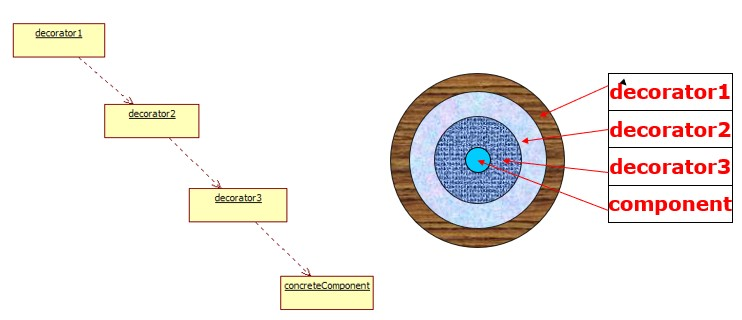
\includegraphics[width=0.85\textwidth]{22_2.jpg}
\end{figure}
%
在具体实现时,要注意以下几点:
\begin{itemize}
  \item 一个装饰类的接口必须与被装饰类的接口相容;
  \item 尽量保持Component作为一个“轻”类;
  \item 如果35有一个ConcreteComponent类,而没有抽象的Component类,则可以把Decorator作为ConcreteComponent的子类;如图:
    \begin{figure}[H]
      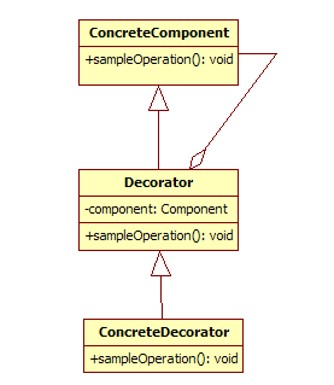
\includegraphics[width=0.35\textwidth]{22_3.jpg}
    \end{figure}
  \item 若只有一个ConcreteDecorator类,则没必要建立一个单独的Decorator类。如图:
    \begin{figure}[H]
      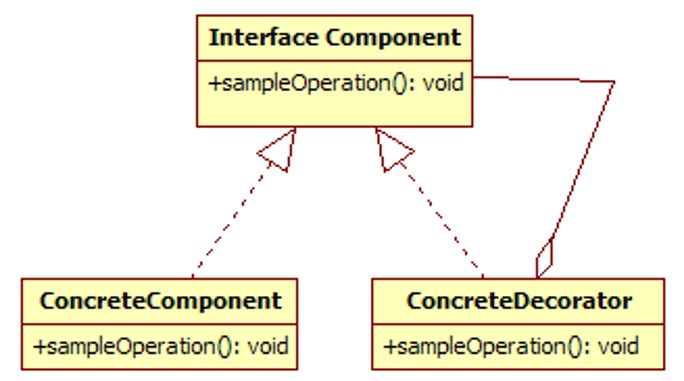
\includegraphics[width=0.45\textwidth]{22_4.jpg}
    \end{figure}
\end{itemize}
%
\textbf{透明性的要求}:
不能向客户端“暴露”装饰对象的具体类型,如下列代码所示:
%
\begin{lstlisting}[language=java]
Component c=new ConcreteComponent();
Component c1=new ConcreteDecorator1(c);
Component c2=new ConcreteDecorator2(c1);
\end{lstlisting}
%
而下面的做法是不对的: \\
\texttt{ConcreteDecorator1 c1=new ConcreteDecorator1();}

\noindent 这就是前面所说的,装饰模式对客户端是完全透明的含义.
因此, ConcreteDecorator里不能有Component类中没有
的公有方法.
%
\subsection{实例:发票系统}
\textbf{要求}:有一个电子销售系统需要打印出顾客的购物发票。一张发票可以分为三个部分:
%
\begin{itemize}
  \item 发票头部(Header):上面有顾客的名字,销售的日期;
  \item 发票主部:销售的货物清单,包括商品名字、购买的数量、单价、小计;
  \item 发票尾部:总金额
\end{itemize}
%
发票的头部、尾部可能有多种形式;要求系统能以灵活的方式更换头、尾,可以灵活
地组合头部尾部,形成新的发票。
%
\begin{figure}[H]
  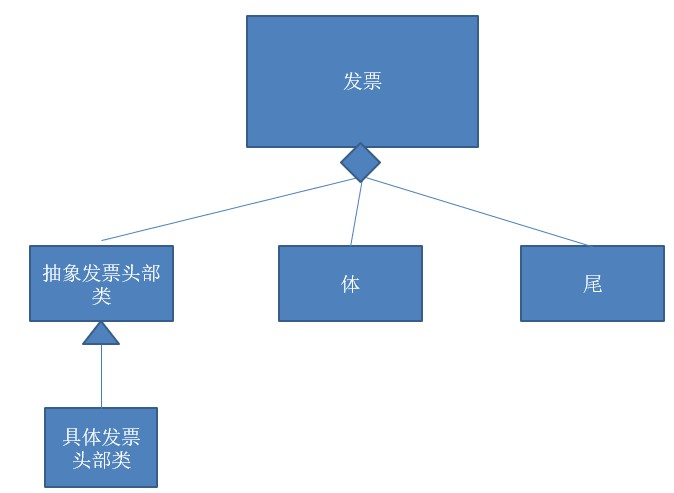
\includegraphics[width=0.55\textwidth]{22_5.jpg}
  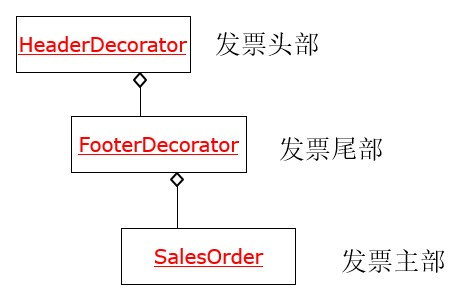
\includegraphics[width=0.45\textwidth]{22_6.jpg}
\end{figure}
%
发票系统的类图:
%
\begin{figure}[H]
  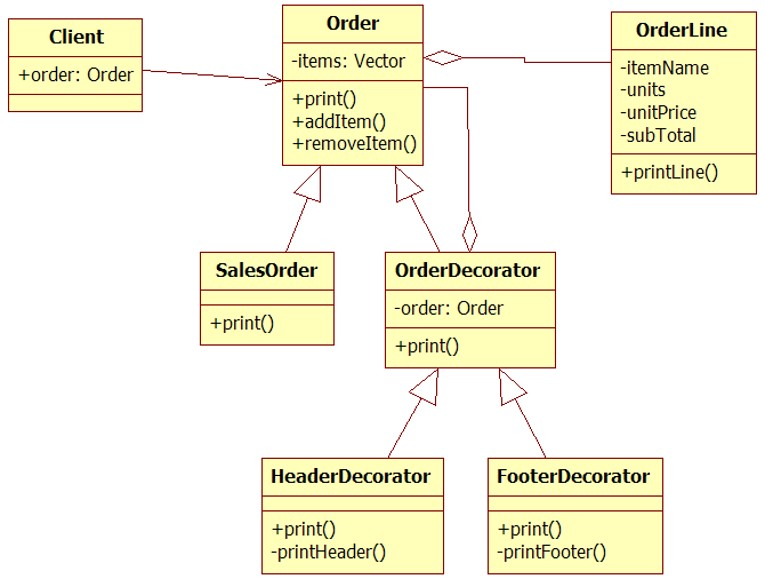
\includegraphics[width=0.55\textwidth]{22_7.jpg}
\end{figure}
%
\lstinputlisting[language=java]{./code/22/2/Order.java}
\lstinputlisting[language=java]{./code/22/2/SalesOrder.java}
\lstinputlisting[language=java]{./code/22/2/OrderDecorator.java}
\lstinputlisting[language=java]{./code/22/2/HeaderDecorator.java}
\lstinputlisting[language=java]{./code/22/2/FooterDecorator.java}
\lstinputlisting[language=java]{./code/22/2/Client.java}
\end{document}
